\documentclass[pdftex,10pt,a4paper,journal]{article}
%\usepackage{nips_2016}
\usepackage{blindtext}
\usepackage{graphicx}
\usepackage{subfiles}
\usepackage{amsmath}
\usepackage{amsthm}
\usepackage{tikz}
\usepackage{wrapfig}
\usepackage{lscape}
\usepackage{rotating}
\usepackage{epstopdf}
\usepackage{subcaption}
\usepackage{multirow}
\usepackage{multicol}
\usepackage[font=small,labelfont=bf]{caption}
\usepackage{hyperref}
\usepackage{capt-of}
\usepackage{pdflscape}
\usepackage{afterpage}
\usepackage{color}
\usepackage{algorithm}% http://ctan.org/pkg/algorithms
\usepackage{algpseudocode}% http://ctan.org/pkg/algorithmicx
\hypersetup{
    colorlinks=true,
    linkcolor=blue,
    citecolor=blue
}
\theoremstyle{definition}
\newtheorem{definition}{Definition}[section]
\newtheorem{theorem}{Theorem}[section]
\newtheorem{lemma}[theorem]{Lemma}
\theoremstyle{remark}
\newtheorem*{remark}{Remark}
\usepackage{amssymb}
\usepackage{amsfonts}
\usepackage{mathtools}
\usepackage{geometry}
 \geometry{
 a4paper,
 total={210mm,297mm},
 left=20mm,
 right=20mm,
 top=20mm,
 bottom=20mm,
 }
\usepackage{multicol}
\usepackage{enumitem}
\setlength{\columnsep}{1cm}
\newcommand{\defeq}{\vcentcolon=}
\newcommand{\eqdef}{=\vcentcolon}
\newcommand*{\V}[1]{\mathbf{#1}}%
\newcommand{\norm}[1]{\left\lVert#1\right\rVert}
\newcommand{\justif}[2]{&{#1}&\text{#2}}
\newcommand{\qedwhite}{\hfill \ensuremath{\Box}}
\newcommand\given[1][]{\:#1\vert\:}
\newcommand{\me}{\mathrm{e}}
\DeclarePairedDelimiterX{\infdivx}[2]{(}{)}{%
  #1\;\delimsize\|\;#2%
}
\DeclarePairedDelimiter\abs{\lvert}{\rvert}%
\newcommand{\Conv}{\mathop{\scalebox{1.5}{\raisebox{-0.2ex}{$\ast$}}}}%
\newcommand{\infdiv}{\infdivx}
\newcommand\tab[1][1cm]{\hspace*{#1}}
\newcommand{\parder}[2]{\frac{\partial{#1}}{\partial{#2}}}
\renewcommand{\qed}{\hfill\blacksquare}
\newcommand*\mean[1]{\bar{#1}}
\hyphenation{op-tical net-works semi-conduc-tor tech-no-lo-gy par-ti-cu-lar}
%\font\myfont=cmr12 at 18pt

\usepackage[acronym]{glossaries}

%use \acrlong, \acrshort, \acrfull
\newacronym{gp}{GP}{Gaussian Process}
\newacronym{gmm}{GMM}{Gaussian Mixture Model}
\newacronym{hmm}{HMM}{Hidden Markov Model}
\newacronym{lstm}{LSTM}{Long Short-Term Memory}
\newacronym{ar}{AR}{Autoregressive}
\newacronym{nn}{RNN}{Neural Network}
\newacronym{rnn}{RNN}{Recurrent Neural Network}
\newacronym{ml}{ML}{Machine Learning}
\newacronym{mlp}{MLP}{Multi-Layer Perceptron}
\newacronym{mse}{MSE}{Mean Squared Error}
\newacronym{gpar}{GP$_{AR}$}{Autoregressive Gaussian Process}
\newacronym{gpatt}{GP$_{att}$}{Attractor-based Gaussian Process}
\newacronym{lstmar}{LSTM$_{AR}$}{Autoregressive LSTM}
\newacronym{lstmatt}{LSTM$_{att}$}{Attractor-based LSTM}

%\begin{titlepage} 
\begin{center}

% Upper part of the page. The '~' is needed because \\ % only works if a paragraph has started. 
\includegraphics[width=0.15\textwidth]{./logo}~\\[1cm]

\textsc{\LARGE Transfer of Status Report}\\[2cm]

\includegraphics[width=0.35\textwidth]{./figs/logo.png}\\[2cm]
% Author and supervisor 

{
\Large 
\textbf{Bernardo Pérez Orozco}\\
\textsl{Balliol College\\
University of Oxford\\}
}
\vspace{15mm}
{
\Large
\par\textbf{Supervised by:}
\par\textsl{Prof. Stephen Roberts}
\vfill
}
% Bottom of the page 
{\large 
\textsc{Doctor of Philosophy in Engineering Sciences\\}
}
{\large
\textsl{August $30^{th}$ 2016}
}

\end{center} 
\end{titlepage}


\title{\huge LSTMs for time series forecasting }
\author{Bernardo P\'erez Orozco\\University of Oxford\\\texttt{ber@robots.ox.ac.uk} \and Stephen J. Roberts\\University of Oxford\\\texttt{sjrob@robots.ox.ac.uk}}

\begin{document}

\maketitle


\begin{abstract}
    \acrshort*{lstm}s are a recent development in the deep neural networks literature that have seen unprecedented success in sequence classification problems, such as speech recognition and image caption generation. Nevertheless, there exists little work on time series forecasting using this type of neural network. In this article, we use \acrshort*{lstm}s to solve time series prediction problems and then benchmark them against another state-of-the-art model, the \acrlong*{gp}. The comparison is with reference to two desirable features of time series models: accurate, long-term forecasting and honest computing. We show that \acrshort*{gp}s still greatly outperform \acrshort*{lstm}s with reference to these desirable aspects.
\end{abstract}

\begin{multicols}{2}
\section{Introduction}
Time series forecasting lies at the heart of much development in the \acrfull*{ml} community. Application domains are broad and ubiquitous: environment quantification, acoustic signal synthesis, stock market prediction, stellar activity modelling and many more. Therefore it is crucial that efficient and accurate time series forecasting models continue to be refined.
\par One recent development in the \acrshort*{ml} community is the \acrfull*{lstm}, which is a special case of the \acrfull*{rnn}. \acrshort*{rnn}s are neural network topologies whose layers form loops. This naturally enables them to model dynamical systems. However, \acrshort*{rnn}s have long been known to be difficult to train by gradient descent \cite{Pascanu2012}. \acrshort*{lstm}s are able to overcome this problem by means of a gating mechanism that allows error signals to be backpropagated for longer periods of time and thus are able to learn long-term dependencies.
\par \acrshort*{lstm}s have improved the state-of-the-art performance in many sequence learning tasks, namely speech recognition \cite{Graves2013,Beaufays2014}, scene labelling \cite{Long2014} and machine translation \cite{Sutskever2014}. Nevertheless, to the authors' knowledge, there is little work on time series prediction using \acrshort*{lstm}s: \cite{Gers2002} first compared them against time-window Multilayer Perceptrons. They have also been benchmarked in domain-specific prediction tasks, such as short-term traffic flow prediction \cite{Tian2015}, where they were compared against SVMs and Stacked Autoencoders. 
\par However, to the authors' best knowledge, there is no recent work that addresses a broad and thorough comparison between LSTMs and other state-of-the-art models. In particular, we are interested in comparing LSTMs with Gaussian Processes (GPs), a model that has recently been shown to outperform other approaches in regression tasks, while also naturally incorporating probabilistic reasoning, i.e. giving confidence intervals for its own predictions. In this work, model performance will be evaluated in terms of accurate and honest, long-term and efficient forecasting.
\par This rest of this article is outlined as follows: in Section \ref{sec_models} we introduce LSTMs and GPs, along with two different approaches to make time series prediction: autoregressive and attractor-based forecasting. Then, in Section \ref{sec_metho} we give an account of our benchmarking methodology; namely, we introduce the performance measures, datasets and architectures that compound our analysis. In the last part of this section we also present and discuss our results. Finally, we mention some conclusion and future work in Section \ref{sec_conc}.


\section{Model Definition}\label{sec_models}
In this section, we give formal definitions for the benchmarked models: LSTMs and GPs. We also discuss how we can allow LSTMs to give an uncertainty estimate for their predictions. Finally, we show how LSTMs and GPs can be used for time series forecasting.

\subsection{Long Short-Term Memory} \label{sub:lstm}
\par Neural Networks are learning models composed of successive layers, each of which is a transformation of its input. Deep learning models, and in particular deep neural networks, are those that contain a large number of layers, usually ranging between 5 and 20 \cite{Szegedy,Simonyan2015}. 
\par One of the recently developed deep learning layers for sequence learning is the \acrlong*{lstm}. The LSTM \cite{Gers2002,Hochreiter1997} is a gated recurrent neural network layer that maps an input vector $\V{x}'_t$ to an output vector $\V{h}_t$, also called the activations of the layer. The input $\V{x}'_t$ is the concatenation of an observation $\V{x}_t$ and the output of the LSTM at time $t-1$, given by $\V{h}_{t-1}$, i.e. $\V{x}'_t = [ \V{x}_t, \V{h}_{t-1} ]$. The output $\V{h}_t$ of an LSTM is given by the element-wise product:
\begin{align*}
    \V{h}_t &= \V{o}_t \odot \tanh(\V{C}_t)
\end{align*}
where $\V{C}_t$ is the \textit{memory cell} at time $t$ and is given by:
\begin{align*}
    \V{C}_t &= \V{i}_t\odot\V{S}_t + \V{f}_t\odot\V{C}_{t-1}\\
    \V{S}_t &= \tanh(\V{W}_S\V{x}'_t + \V{b}_S)
\end{align*}
\par in which $\V{i}_t, \V{o}_t, \V{f}_t$ are the input, output and forget gates respectively, given by:
\begin{align*}
    \V{i}_t &= \sigma(\V{W}_i\V{x}'_t + \V{b}_i)\\
    \V{o}_t &= \sigma(\V{W}_o\V{x}'_t + \V{b}_o)\\
    \V{f}_t &= \sigma(\V{W}_f\V{x}'_t + \V{b}_f)
\end{align*}
where $\sigma$ is the sigmoid function. Hence the learnable parameters $\theta$ of an LSTM layer are given by the union of $\{\V{W}_i, \V{W}_o, \V{W}_f, \V{W}_S\}$ and the bias vectors $\{\V{b}_i, \V{b}_o, \V{b}_f, \V{b}_S\}$.
\par It is often useful to think of RNN architectures in an unfolded fashion, as can be seen in Figure \ref{fig:rnn}. The results of the equations above travel through the vertical arrows in order to compute the output at time $t$, $\V{h}_t$. Then, $\V{h}_t$ itself is propagated through the horizontal arrows as an input to compute $\V{h}_{t+1}$.
\par It is important to remark that the output of an LSTM is always constrained to the range $(-1, 1)$ since $\V{h}_t$ is given by the product of vectors that have been squashed by either a sigmoid or a hyperbolic tangent function. Therefore, in order to use LSTMs for time series prediction outside this range, we can use a linear dense layer at each LSTM timestep. The output of a linear dense layer $\V{h}_t^{(\text{dense})}$ for an input $\V{x}$ is given by an additional linear transformation:
\begin{align*} 
    \V{h}_t^{(\text{dense})} = \V{W}_{\text{dense}}\V{x} + \V{b}_{\text{dense}}
\end{align*}
\par Neural networks are trained by minimising a loss function $\mathcal{L}$. The most widespread optimisation method in the neural network community is gradient descent, which finds an optimal solution in an iterative fashion:
\begin{align*}
    \theta_{t+1} = \theta_{t} - \alpha \nabla_\theta \mathcal{L}(\theta) 
\end{align*}
where $\alpha$ is the learning rate. Recent developments in gradient descent include: 
\begin{itemize}
\item \textbf{Minibatch stochastic gradient descent}. It allows for multiple updates per dataset epoch by using gradient estimates from taking random, small subsets of the data \cite{Bottou2010}. The approximate gradient is computed as the empirical mean of the gradient evaluated at each individual data point in the minibatch.
\item \textbf{Adaptive learning rate.} These methods enable the learning rate to adapt automatically over time, normally considering information unveiled by previous gradient computations. AdaGrad (Adaptive Gradient) \cite{Duchi2011} was the pioneer in this class of techniques. Let $g_\tau$ be the approximate gradient at time $\tau$, and let $G_i=\sum_{\tau=1}^t g_{\tau, i}^2$. Then the update for the i-th parameter $\theta_i$, using a smoothing factor $\epsilon$ and initial learning rate $\alpha$, is given by:
    \begin{align*}
        \theta_{t+1, i} = \theta_{t, i} - \frac{\alpha}{\sqrt{G_i + \epsilon}}g_{t, i}
    \end{align*}
\item \textbf{Momentum} computes a new update $\nu_t$ using not only the gradient at time $t$, but also previous updates $\nu_{t-1}, ..., \nu_1$ \cite{Ruder2015}, i.e. if $\theta_{t+1} = \theta_t - \nu_t$, then allow $\nu_t = \gamma\nu_{t-1} + \alpha\nabla_\theta L(\theta)$, where $\gamma$ is called the momentum factor.
\end{itemize}
 \par Two of the most successful methods that incorporate some of these developments are Adam and RMSProp \cite{Kingma2014}. Although they all have a similar performance \cite{Kingma2014}, Adam is the one that has shown the best empirical results so far. Adam stands for Adaptive Moment Estimation, where moment in this case refers to the bias-corrected estimates of the first- and second-order moments of the gradient. Adam keeps an exponentially decaying sum of gradients that emulates the performance of momentum. The update equations are given below:

\begin{align*}
    \theta_{t+1} &= \theta_t - \frac{\alpha}{\sqrt{\hat{v_t}} + \epsilon}\hat{m_t}\\
    \hat{m_t} &= \frac{1}{1 - \beta_1^t}\beta_1 m_t\\
    \hat{v_t} &= \frac{1}{1 - \beta_2^t}\beta_2 v_t\\
    m_t &= \beta_1m_{t-1} + (1 - \beta_1)g_t\\
    v_t &= \beta_2v_{t-1} + (1 - \beta_2)g_t^2
\end{align*}
where $\beta_1, \beta_2 \in (0, 1)$ are called the bias-correction hyperparameters, with default values $\beta_1 = 0.9, \beta_2 = 0.999$. Any of the gradient descent variants mentioned so far can be used to train LSTMs given that gradients can be computed efficiently and accurately. LSTMs are widely regarded as the succesors of the more general RNNs, which suffered from the vanishing gradient problem. For more information on this, refer to Appendix A.

\par In regard to software implementations, there exists a variety of packages that allow for agile development of Deep Learning models. Three of the most widely used are Theano \cite{Bergstra2010,Bastien2012}, Torch \cite{Collobert2011} and Tensorflow \cite{tensorflow}. Another example is Keras \cite{chollet2015keras}, which can use Theano or Tensorflow as a backend but whose syntax is more similar to Torch or MATLAB.

\par With reference to applications, LSTMs have been used extensively for classification problems, but to the authors' best knowledge, little work has been done for time series prediction problems. Some domain-specific applications of LSTMs for sequences with continuous values include a system for robotic heart surgery that learns how to tie knots \cite{Mayer2008}; interval timing for reproducing dopamine activity \cite{Rivest2010}; and stock return predictions \cite{ZacharyC.Lipton2015}. In all cases, the authors identify domain-specific advantages that allow for efficient modelling using LSTMs

\begin{figure*}[t]
    \centering
    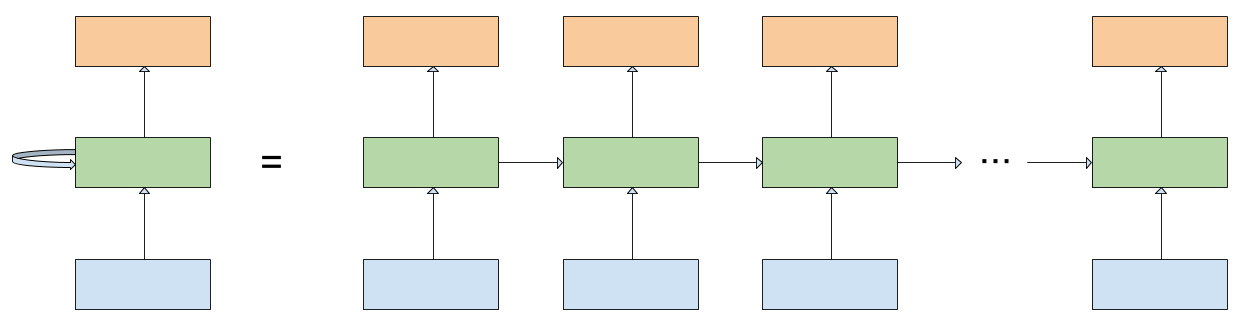
\includegraphics[width=\textwidth]{figs/rnn.png}
    \caption{Recurrent neural networks have at least one directed cycle, often present in the form of a self-connected layer. The resulting graph and be unfolded as a grid, which enables sequence learning to be visualised more clearly.}
    \label{fig:rnn}
\end{figure*}

%\subsubsection{LSTMs for time series forecasting}
%In this section, we give an account of the existing literature of \acrshort*{lstm}s for time series forecasting.  
%\par In \cite{Tian2015}, LSTMs were used to predict short-term traffic flow and outperformed other methods (Support Vector Machines, Random Walks and Stacked Autoencoders) in terms of accuracy metrics such as Mean Absolute Percentage Error (MAPE) and Root Mean Squared Error (RMSE).
%\par In a similar fashion, \textbf{cite} demonstrates the use of LSTMs to predict the quality of user contributions in Wikipedia. The authors use handcrafted features and evaluate their system against other neural network models. Crucially, their best results are obtained using a combined approach that stacks an additional fully connected layer on top of the LSTM layer. This suggests that LSTM-based time series forecasting can be improving by using deeper architectures.

%\par To the authors' best knowledge, there is no recent work that presents a thorough comparison between LSTMs and other state-of-the-art models, and crucially none that aims at a broad benchmarking of models, i.e. one that also considers their time and memory complexities. Such comparison is necessary if we are to account for the accuracy-performance trade-off present in some tasks.

\subsection{Gaussian Process}
A Gaussian Process (GP) is a generalisation of the Gaussian distribution to infinite dimensional spaces.  It is defined as a collection of random variables such that any of its finite subsets has a joint Gaussian distribution that is completely defined by its mean and covariance (also called kernel) functions $m(\V{x}), k(\V{x}, \V{x}')$. In time series prediction, our random variables are functions $f(\V{x})$ evaluated at a location $\V{x}$. A GP's mean and covariance functions are defined as:
\begin{align*}
    m(\V{x}) &= \mathbb{E}[f(\V{x})]\\
    k(\V{x}, \V{x}') &= \mathbb{E}[(f(\V{x}) - m(\V{x}))(f(\V{x}') - m(\V{x}'))]
\end{align*}

\par Some of the most used kernels in Machine Learning \cite{Rasmussen2006} are the Squared Exponential or Radial Basis Function (RBF) and Mat\'ern with $\nu = 5/2$ and $\nu = 3/2$. For two points located $r$ units apart, these kernels are given by:
\begin{align*}
    k_{\text{RBF}}(r) &= \exp{\left(-\frac{r^2}{2\ell^2}\right)}\\
    k_{\nu = 3/2}(r) &= \left( 1 + \frac{\sqrt{3}r}{\ell}\right) \exp{\left(-\frac{\sqrt{3}r}{\ell}\right)} \\ 
    k_{\nu = 5/2}(r) &= \left( 1 + \frac{\sqrt{5}r}{\ell} + \frac{5r^2}{3\ell^2}\right) \exp{\left(-\frac{\sqrt{5}r}{\ell}\right)} 
\end{align*}
where $\ell$ is the characteristic length-scale of the process. 

\par When choosing a kernel it is often important to look at its differentiability properties. A process $f(\V{x})$ is said to be \textbf{continuous in mean square} at $\V{x}_*$ if $\mathbb{E}[f(\V{x}_k - f(\V{x}_*))] \rightarrow 0$ as $k \rightarrow \infty$ \cite{Rasmussen2006}. Then we can define the mean square (MS) derivative of $f(\V{x})$ in the direction of the $i$-th standard vector $\V{e}_i$ in the usual way:

\begin{align*}
    \frac{\partial f(\V{x})}{\partial{x_i}} = \lim_{h\rightarrow 0} \frac{f(\V{x} + h\V{e}_i) - f(\V{x})}{h}
\end{align*}

when the limit exists. 

\par A GP with an RBF kernel is infinitely MS differentiable and thus is able to accurately fit very smooth data. However it has been pointed out \cite{Stein1999} that some processes may not satisfy this smoothness assumption and instead recommend using the Mat\'ern kernels, which are only differentiable a finite amount of times depending on the value of $\nu$ and can therefore model more rough data. This flexibility makes both types of kernels be able to model a wide range of scenarios and will thus we will use them later in our experiments.

\par A GP defines a distribution of functions to choose from. In particular, training a GP means setting out initial beliefs about a problem, encapsulated by a so-called \textit{GP prior}, and adapting them as we see data. The result is called the \textit{GP posterior}. The \textit{posterior mean} can then be used as the most likely forecast for our time series.

\par The following presentation is based on the presentation given in \cite{Rasmussen2006}. In order to perform prediction using a GP, we need to adjust the prior beliefs. In particular, consider a set of $n$ noise-free observed points $\{\V{X}, \V{f}\}$ and a set of $n_*$ test points $\{\V{X}_*, \V{f}_*\}$. By definition of the GP, the joint distribution of a finite subset of function values is given by a multivariate normal. Let $\V{f}, \V{f}^*$ be the function values at each of the $n+n_*$ training and test locations. Then, assuming a zero mean prior, the GP prior is given by:

\begin{align*}
    \begin{bmatrix}
           \V{f} \\
           \V{f}_* \\
    \end{bmatrix} &\sim \mathcal{N}\left(\V{0}, 
                                        \begin{pmatrix}
                                        K(\V{X}, \V{X}) & K(\V{X}, \V{X}_*)\\
                                        K(\V{X}_*, \V{X}) & K(\V{X}_*, \V{X}_*)
                                        \end{pmatrix}\right)
\end{align*}

where $K(\V{X}, \V{X}_*)$ denotes the covariance matrix as calculated using the kernel $k$ between each pair of training and test points. The submatrices $K(\V{X},\V{X}), K(\V{X}_*, \V{X}), K(\V{X}_*, \V{X}_*)$ are computed analogously. In this context, transforming the GP prior into the GP posterior by conditioning $\V{f}_*$ on the observed values $\V{f}$. Using properties of the Gaussian \cite{Rasmussen2006}, it can then be shown that the posterior distribution after conditioning on the observed data $\V{f}$ is given by:

\begin{align*}
    \V{f}_*|\V{X}_*, \V{X}, \V{f} \sim \mathcal{N}(K(\V{X}_*, \V{X})K(\V{X},\V{X})^{-1}\V{f}, \\K(\V{X}_*, \V{X}_*) - K(\V{X}_*, \V{X})K(\V{X}, \V{X})^{-1}K(\V{X}, \V{X}_*))
\end{align*}


\par We can see that Gaussian Processes are naturally endowed with probabilistic reasoning: the \textit{posterior variance} allows them to give estimates of the variance of $f(\V{x}_*)$ at each location $\V{x}_*$, i.e. they are able to produce ``error bars' that naturally speak about the uncertainty of their predictions.

\par When working with noisy observations, and assuming the noise is additive Gaussian with variance $\sigma_n^2$, we can adjust the GP prior as:

\begin{align*}
    \begin{bmatrix}
           \V{f} \\
           \V{f}_* \\
    \end{bmatrix} &\sim \mathcal{N}\left(\V{0}, 
                                        \begin{pmatrix}
                                        K(\V{X}, \V{X}) + \sigma_n^2+I & K(\V{X}, \V{X}_*)\\
                                        K(\V{X}_*, \V{X}) & K(\V{X}_*, \V{X}_*)
                                        \end{pmatrix}\right)
\end{align*}

\par By conditioning $\V{f}_*$ on $\V{f}$ and carrying out a similar derivation, we get the posterior mean and variance for the noisy observations case:

\begin{align*}
    \V{f}_*|\V{X}_*, \V{X}, \V{f} &\sim \mathcal{N}(\V{\mean{f}}_*, \Sigma_{*}),\\
    \V{\mean{f}}_* &= K(\V{X}_*, \V{X})[K(\V{X},\V{X})^{-1} + \sigma_n^2I]\V{f},\\
    \Sigma_* &= K(\V{X}_*, \V{X}_*) - \\&K(\V{X}_*, \V{X})[K(\V{X}, \V{X})^{-1} + \sigma_n^2I]K(\V{X}, \V{X}_*)
\end{align*}

With respect to software implementations, the Python package GPy \cite{gpy2014} offers an implementation that accounts for many of the most widely used kernels (including the RBF and Mat\'ern), as well as efficient implementations of algorithms for GP optimisation.

\subsection{Neural networks with error bars} \label{sub_nnerror}
The parameters $\theta$ of a neural network are a minimum point of a loss function $\mathcal{L}$, which for regression tasks is often the $L_2$-regularised Minimum Squared Error (MSE), given by:
\begin{align*}
    \mathcal{L}(\theta) = \frac{1}{2M}\sum_{i=1}^M(\V{Y}_i - \V{\hat{Y}}_i)^2 + \lambda\sum_{w \in \theta}\norm{w}^2
\end{align*}
where $\V{Y}, \V{\hat{Y}}$ are the ground truth and predictions respectively, and $\lambda$ is called the regularisation hyperparameter.
\par This loss function is increasingly non-linear as the number of layers in the network grows, and hence contains a vast number of minima. Since neural networks are often trained by stochastic gradient descent, the quality of the obtained result heavily depends on the optimisation method's initialisation conditions.
\par One way to endow neural networks with error bars is by performing a more careful search through the loss function's landscape. In particular, consider optimising $\mathcal{L}$ a number $N'$ of times, each time under different initialisation conditions. This will yield a set of $N'$ minima drawn from $\mathcal{L}$, each of which can produce a forecast $\V{\hat{Y}}^{(n')}$ from our dataset. Then, the set $\{\V{\hat{Y}}^{(1)}, \V{\hat{Y}}^{(2)}, ..., \V{\hat{Y}}^{(N')}\}$ forms an empirical posterior predictive distribution whose statistics approach the true posterior's as $N'$ grows larger. In particular, the empirical mean can be used as a single forecast $\V{\hat{Y}}$ with standard deviation given by the empirical standard deviation $\sigma_{\V{\hat{Y}}}$ of the predictive distribution.

\par Sampling optima by repeated training becomes prohibitive as datasets and input dimensions grow, and therefore finding better ways of attaining such points remains an active area of research that can impact the way in which neural networks reason about their own predictions.

\subsection{Autoregressive and attractor-based forecasting}
In this subsection, we discuss two different approaches to perform time series forecasting using LSTMs or Gaussian Processes. 
\par In the autoregressive approach, we perform one-step prediction from the preceding $K$ samples, i.e. $\V{x}_t = f(\V{x}_{t-1}, \V{x}_{t-2}, ..., \V{x}_{t-K})$. In our setting, $f$ is either an LSTM or a GP. Given a time series $\V{X} = (\V{x}_{1}, \V{x}_{2}, ..., \V{x}_{T})$, a set of $M$ overlapping blocks $\V{X}_{AR} = \{\V{X}_1, \V{X}_2, ..., \V{X}_M\}$ of $K$ samples each can be built by applying a sliding window to $\V{X}$ using a stride $s$.  Likewise, a set of predicted samples $\V{Y}_{AR}$ can be built by windowing the original sequence $\V{X}$ starting from the $(K+1)$-th sample and using the same stride $s$.
\par Another approach in time series forecasting consists in embedding the time series alongside lagged versions of itself into what we call an \textit{attractor embedding}. This embedding is motivated by the observation that the information required to make one-step prediction may not necessarily lie in the last $K$ samples, but rather further away in the past. Let $\V{X}^{(B)}$ be the lagged version of the time series $\V{X}$ by $B$ samples, and construct $\V{X}' = (\V{X}, \V{X}^{(B_1)}, \V{X}^{(B_2)}, ..., \V{X}^{(B_P)})$ by stacking $P$ lagged time series. Then $\V{X}'$ can be windowed in a way analogous to the autoregressive approach into $\V{X}_{att} = \{\V{X}'_1, \V{X}'_2, ..., \V{X}'_M\}$. $\V{Y}_{att}$ can be constructed in a similar fashion.
\par In this work, we will compare the two approaches using both, GPs and LSTMs. Thus we will henceforth refer to \acrshort*{lstmar} and \acrshort*{gpar} to the models trained using the autoregressive approach, and \acrshort*{lstmatt} and \acrshort*{gpatt} to those using the attractor embedding approach.

\section{Benchmarking methodology}\label{sec_metho}

In this section, we set out the experiments to be performed using the models described in Section \ref{sec_models}. Subsection \ref{sub_measures} describes the criteria used to benchmark the models, and subsection \ref{sub_experiments} introduces the benchmarking datasets used in our work.

\subsection{Performance measures} \label{sub_measures}
In our work, we compare the models described in Section \ref{sec_models} with several metrics so as to allow for a holistic benchmarking. In particular, two desirable qualities we evaluate in each model are:
\begin{itemize}
    \item \textbf{Long-term, accurate prediction and timing}. The degree of presence of this property in a model is given by its ability to make accurate forecasts in a timely fashion. As a consequence, the model is able to forecast the presence of critical points, i.e. able to capture the fundamental oscillations of the time series.
    \item \textbf{Honest computing}. In our framework, we value models that are able to predict not only their knowledge, but also their ignorance. In other words, we value models that are able to tell how confident they are about their forecasts. Whereas GPs account for this naturally, LSTMs do not. Instead, we will use the approach proposed in subsection \ref{sub_nnerror}.
    %\item \textbf{Efficiency}. Some models with very high accuracy may also require a vast amount resources to be executed. When such degree of accuracy is not needed, or when the model is to be run under limited amounts of resources, models with less accuracy may be a better choice. We compare models in terms of the time it takes for them to make a one-step prediction once they have been trained, and in terms of the number of parameters they need to do this task.
\end{itemize}

\begin{figure*}[ht] 
    \centering
    \begin{subfigure}[t]{0.5\textwidth}
        \centering
        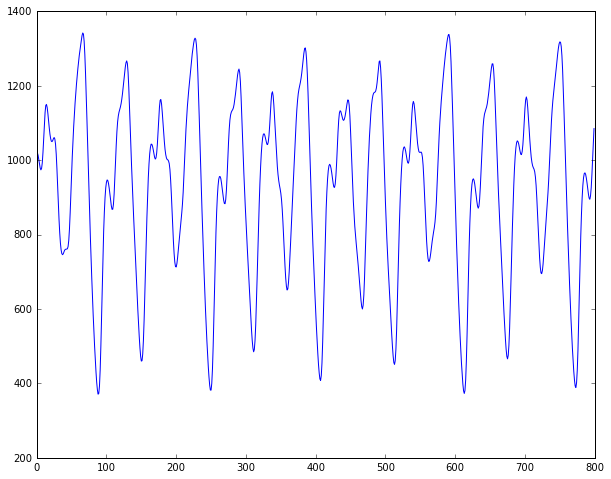
\includegraphics[height=1.2in, width=3.8in]{figs/mg.png}
        \caption{Mackey Glass chaotic time series}
    \end{subfigure}%
    
    \begin{subfigure}[t]{0.5\textwidth}
        \centering
        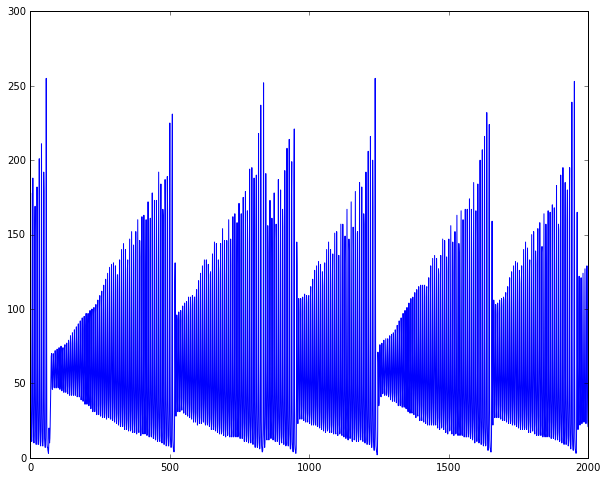
\includegraphics[height=1.2in, width=3.8in]{figs/laser.png}
        \caption{Santa Fe Laser dataset}
    \end{subfigure}
    
    \begin{subfigure}[t]{0.5\textwidth}
        \centering
        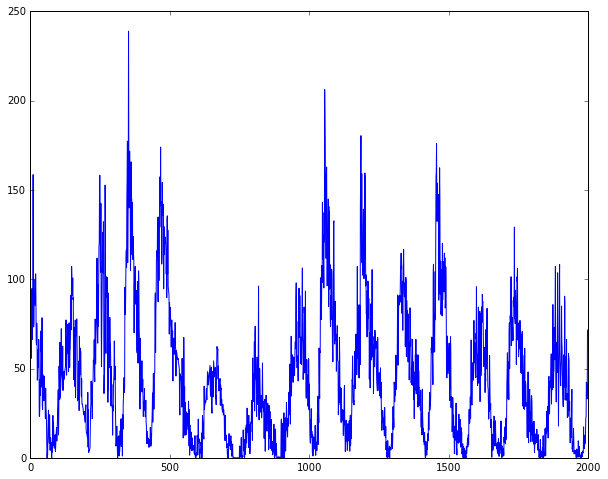
\includegraphics[height=1.2in, width=3.8in]{figs/sunspot.png}
        \caption{Sunspot dataset}
    \end{subfigure}
    \caption{Datasets used for our experiments}\label{fig:datasets}
\end{figure*}

The qualities above will therefore be measured using the following criteria:
\begin{itemize}
    \item \textbf{Normalised \acrlong*{mse} (NMSE)}. This criterion measures accurate and timely forecasting after predicting $M'$ samples $\V{\hat{Y}}$ while also accounting for the variance of the ground truth $\V{Y}$, and is given by:
    \begin{align*}
        \text{NMSE}(\hat{\V{Y}}, \V{Y}) = \frac{\norm{\V{Y} - \V{\hat{Y}}}^2}{\text{var}{(\V{Y})}M'}
    \end{align*}
    
    \item \textbf{Median predictive log-likelihood (MedLL)}. The probability of predicting a sample $\V{Y}_t$ at time $t$ is given by a normal distribution with mean $\V{\hat{Y}}_t$ and variance $\sigma^2_{\V{\hat{Y}}, t}$, i.e. $\V{Y}_t \sim \mathcal{N}(\V{\hat{Y}}_t, \sigma^2_{\V{\hat{Y}}, t})$. Assuming that the samples $\V{\hat{Y}}_1, \V{\hat{Y}}_2, ..., \V{\hat{Y}}_{M'}$ are conditionally independent given the posterior mean and variance $\V{\hat{Y}}, \sigma^2_{\V{\hat{Y}}}$, the median log-likelihood (LL) is then given by the median of the set $\{\log{\mathcal{N}(\V{\hat{Y}}_1, \sigma^2_{\V{\hat{Y}}, 1})}, ..., 
    \mathcal{N}(\V{\hat{Y}}_{M'}, \sigma^2_{\V{\hat{Y}}, M'})\}$
    
    We propose using the median LL (MedLL) because it is less sensitive to outliers than other approaches, such as the mean LL. It can be seen that the mean LL (MLL) is proportional to the joint LL:
    
    \begin{align*}
        \text{MLL}(\V{Y}) &= \frac{1}{M'}\sum_{t=1}^{M'}\log{p(\V{Y}_t | \V{\hat{Y}}_{t}, \sigma^2_{\V{\hat{Y}}, t})} \\
        &\propto \sum_{t=1}^{M'}\log{p(\V{Y}_t | \V{\hat{Y}}_{t}, \sigma^2_{\V{\hat{Y}}, t})} \\
        &= \log{\prod_{t=1}^{M'}p(\V{Y}_t | \V{\hat{Y}}_{t}, \sigma^2_{\V{\hat{Y}}, t})}\\
        &= \log{p(\V{Y}_1, \V{Y}_2, ..., \V{Y}_{M'})}
    \end{align*}
    
    and from this derivation it can also be seen that whenever any $p(\V{Y}_t | \V{\hat{Y}}_{t}, \sigma^2_{\V{\hat{Y}}, t})$ is very close to zero, the resulting MLL will tend to $-\infty$. As a consequence, even models with a very small number of mistakes are heavily penalised by MLL. Instead, we desire to have a metric that favours models as they make a larger number of correct predictions, at which the MedLL succeeds.
    
    %\item \textbf{Mean variance in forecast}. Each forecast sample $\V{\hat{Y}}_j$ is estimated with a variance var$_j$. The mean variance after forecasting $M'$ samples into the future is given by:
    %\begin{align*}
    %    \text{MV}(\text{var}) = \frac{1}{M'}\sum_{j=1}^{M'}\text{var}_j
    %\end{align*}
    \item \textbf{Accuracy rejection curves}. These allow to compare the accuracy of estimators as their acceptance rate decreases. This enables us to see how the accuracy of our models varies as we make them be more strict with their own forecasts.
    
    \par In this context, we accept samples $\V{T}_t$ only when they are drawn with probability $p(\V{T}_t | \V{\hat{Y}}_{t}, \sigma^2_{\V{\hat{Y}}, t}) > \gamma$. Accuracy-rejection curves allow us to see how many samples we accept as $\gamma$ increases, i.e. as we become more strict. 
    
    \par We provide plots for each dataset in order to compare the acceptance/rejection rates of each model. Additionally, from these graphs we also compute the cut-off values of $\gamma_{75\%}, \gamma_{50\%}, \gamma_{25\%}$ for which each model will accept 75\%, 50\% and 25\% of the test samples. Good models have larger values than others for $\gamma_{75\%}, \gamma_{50\%}, \gamma_{25\%}$, as they produce a larger amount of good samples even if they are very strict.
    %\item \textit{Time-efficiency}. This is the time (in milliseconds) the model takes to predict a single sample into the future.
    %\item \textbf{Number of parameters}. This is the number of parameters each model needs to store in order to make a prediction. 
\end{itemize}


\subsection{Datasets} \label{sub_datasets}
In this subsection we introduce the time series datasets used to benchmark our models. These are shown in Figure \ref{fig:datasets}.
\begin{itemize}
    \item\textbf{ Mackey-Glass.} This is a time-delay differential equation of the shape:
    \begin{align*}
        \frac{dx}{dt} = \beta\frac{x_{t-\tau}}{1 + x_{t-\tau}^n} - \gamma x, \gamma, \beta, \tau, n > 0
    \end{align*}
    For different configurations of its parameters, this time series can exhibit a range of quasi-periodic chaotic behaviour.
    \item \textbf{Santa Fe Laser dataset.} These samples represent the fluctuations of a far-infrared laser, approximately described by three coupled nonlinear ordinary differential equations \cite{Weigend1994}.
    \item \textbf{Sunspot data. } Data collected at the Swiss Federal Observatory and the Tokyo Astronomical Observatory. Contains the monthly mean relative sunspot numbers from 1749 to 1983. \cite{Andrews1985}
\end{itemize}
 \par Each dataset was divided in 800, 1000 and 1000 training samples, and 80, 100 and 100 testing samples respectively. 

\subsection{Experiments} \label{sub_experiments}
Following the model description from Section \ref{sec_models}, we fitted 13 different models to each of the datasets described in subsection \ref{sub_experiments}. Our models are listed below:
\begin{itemize}[noitemsep,topsep=0pt]
\item Autoregressive LSTM 
    \begin{itemize}
        \item with 1 layer (50 neurons) and no regularisation
        \item with 4 layers and no regularisation
        \item with 4 layers and $L_2$ regularisation using $\lambda = 0.001$
        \item with 4 layers and $L_2$ regularisation using $\lambda = 0.01$
        \item with 4 layers and $L_2$ regularisation using $\lambda = 0.05$
    \end{itemize}
\item Attractor-based LSTM
    \begin{itemize}
        \item with 4 layers and no regularisation
        \item with 4 layers and $L_2$ regularisation using $\lambda = 0.001$
        \item with 4 layers and $L_2$ regularisation using $\lambda = 0.01$
        \item with 4 layers and $L_2$ regularisation using $\lambda = 0.05$
    \end{itemize}
\item Autoregressive GP
    \begin{itemize}
        \item with the Mat\'ern 3/2 kernel
        \item with the Mat\'ern 5/2 kernel
        \item with the Radial Basis Function kernel
    \end{itemize}
\item Attractor-based GP
    \begin{itemize}
        \item with the Mat\'ern 3/2 kernel
        \item with the Mat\'ern 5/2 kernel
        \item with the Radial Basis Function kernel
    \end{itemize}
\end{itemize}

\par All the LSTM models have a final dense layer for output scaling. The 4-layer LSTMs have layer sizes equal to 35, 20, 10 and 8 neurons respectively. In addition, we have created several instances so as to account for the effect of deeper and regularised networks. In order to be able to produce error bars for LSTMs, we have trained each architecture 100 times and obtained estimates for a mean prediction and variance at each location. Our results are presented in the next subsection.

\begin{figure*}[ht] 
    \centering
    \begin{subfigure}[t]{0.5\textwidth}
        \centering
        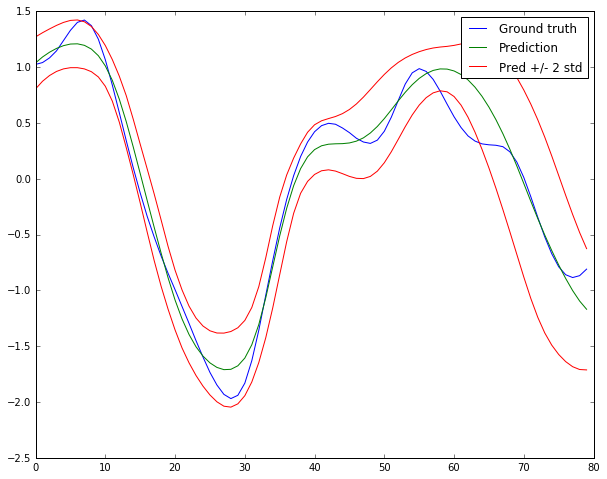
\includegraphics[height=1.8in]{figs/mg_lstm.png}
        \caption{Autoregressive LSTM, 4 layers, No Reg.}
    \end{subfigure}%
    ~ 
    \begin{subfigure}[t]{0.5\textwidth}
        \centering
        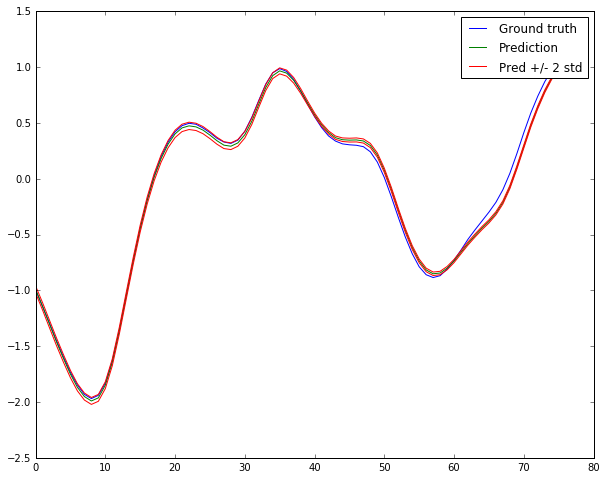
\includegraphics[height=1.8in]{figs/mg_gpatt52.png}
        \caption{Attractor GP, Mat\'ern 5/2 Kernel}
    \end{subfigure}

    \begin{subfigure}[t]{0.5\textwidth}
        \centering
        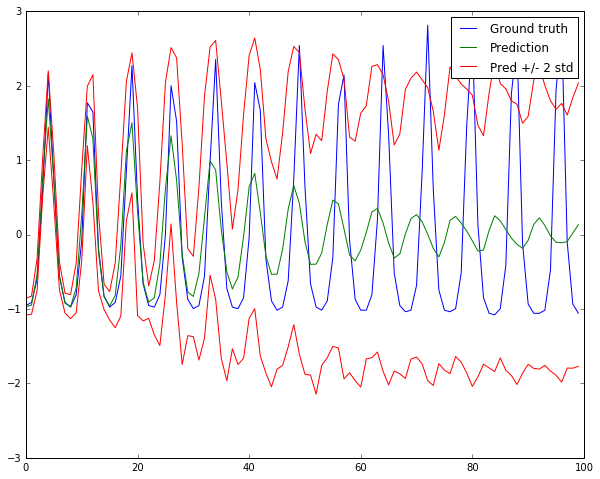
\includegraphics[height=1.8in]{figs/laser_lstm.png}
        \caption{Autoregressive LSTM, 4 layers, No Reg}
    \end{subfigure}%
    ~ 
    \begin{subfigure}[t]{0.5\textwidth}
        \centering
        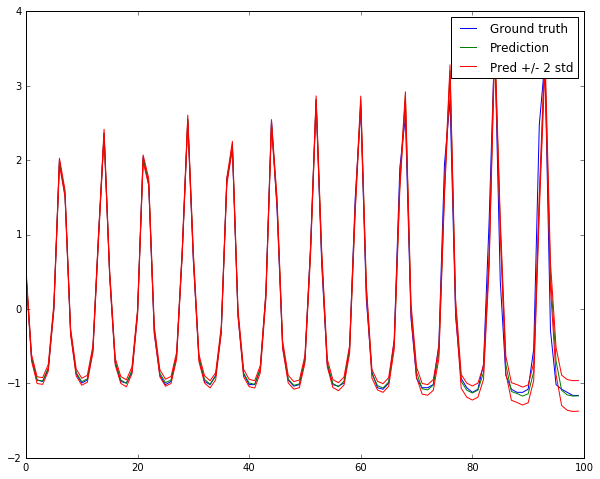
\includegraphics[height=1.8in]{figs/laser_gpatt52.png}
        \caption{Attractor GP, RBF Kernel}
    \end{subfigure}

    \begin{subfigure}[t]{0.5\textwidth}
        \centering
        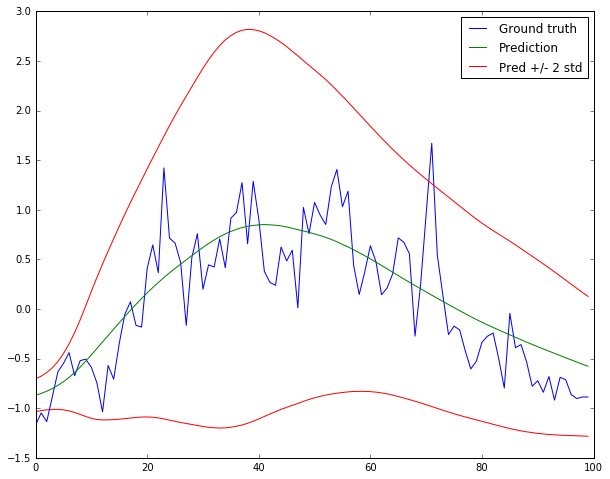
\includegraphics[height=1.8in]{figs/sunspot_lstm.png}
        \caption{Autoregressive LSTM, 4 layers, Reg $\lambda = 0.001$}
    \end{subfigure}%
    ~ 
    \begin{subfigure}[t]{0.5\textwidth}
        \centering
        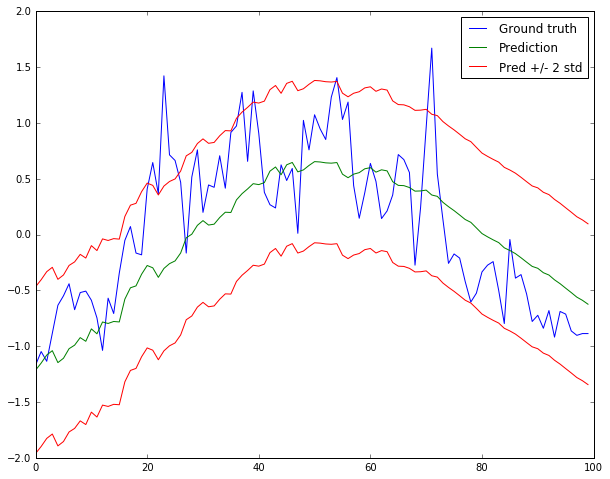
\includegraphics[height=1.8in]{figs/sunspot_gp32.png}
        \caption{Autoregressive GP, RBF Kernel}
    \end{subfigure}
    \caption{Best LSTM and GP predictions for the Mackey-Glass (top), Laser (middle) and Sunspot (bottom) datasets}\label{fig:bestpreds}
\end{figure*}

\begin{figure*}[ht] 
    \centering
    \begin{subfigure}[t]{0.5\textwidth}
        \centering
        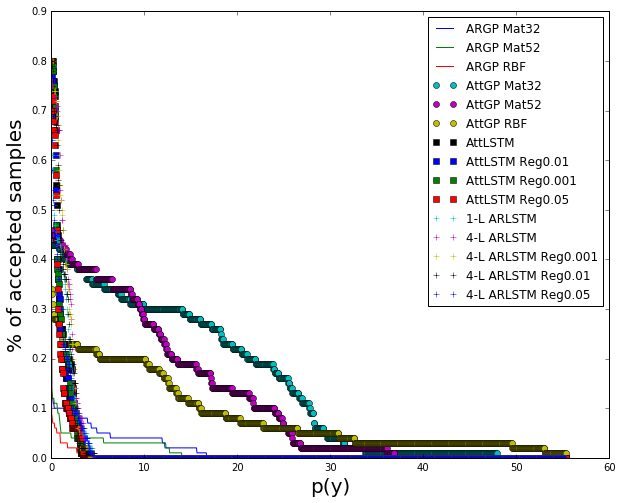
\includegraphics[height=3in, width=3in]{figs/accrej_mg.png}
        \caption{Acceptance-rejection curve for the Mackey-Glass dataset}
    \end{subfigure}%
    
    \begin{subfigure}[t]{0.5\textwidth}
        \centering
        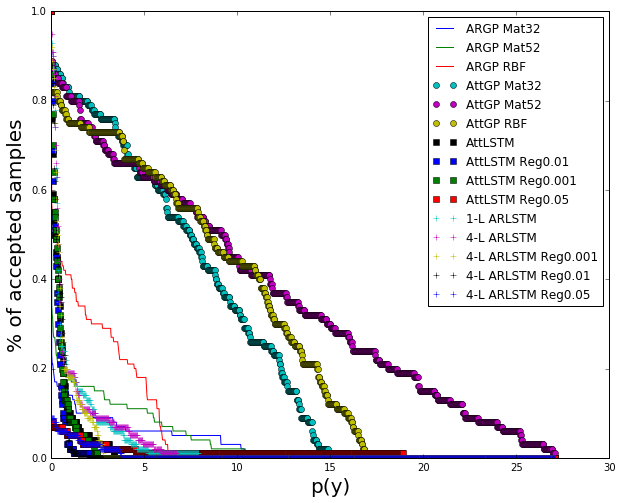
\includegraphics[height=3in, width=3in]{figs/accrej_laser.png}
        \caption{Acceptance-rejection curve for the Laser dataset}
    \end{subfigure}
    
    \begin{subfigure}[t]{0.5\textwidth}
        \centering
        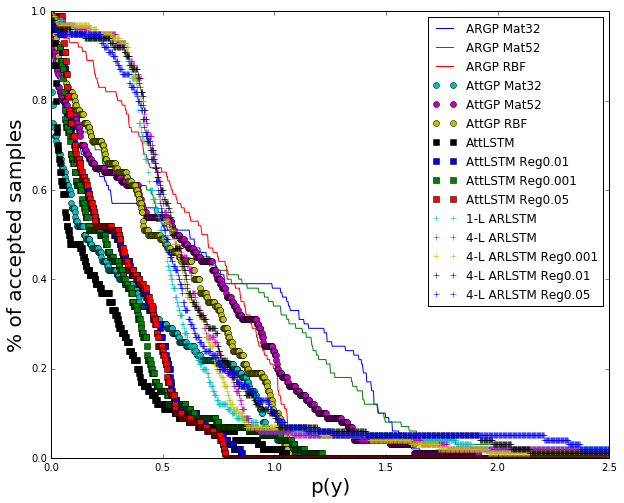
\includegraphics[height=3in, width=3in]{figs/accrej_sunspot.png}
        \caption{Acceptance-rejection curve for the Sunspot dataset}
    \end{subfigure}%
    
    \caption{Acceptance-rejection curves for all three experiments.}\label{fig:accrej}
\end{figure*}


\subsection{Results} \label{sub_res}
Tables \ref{tab:mg}, \ref{tab:laser} and \ref{tab:sunspot} show the results obtained after fitting the models introduced in subsection \ref{sub_experiments} to the datasets presented in subsection \ref{sub_datasets}. The last 100 training samples in each dataset were used as a seed to forecast the next 80, 100 and 100 testing samples (respectively) in a one-step prediction fashion, i.e. appending each newly predicted sample, and using them in conjunction with the seed to perform the next prediction successively. 
\par Each model was then measured in terms of the performance measures described in subsection \ref{sub_measures}. Figure \ref{fig:bestpreds} compares the ground truth against the most accurate mean prediction obtained in each family of models. Finally, the acceptance/rejection curves are shown in Figure \ref{fig:accrej}. 

\par From the results tables we can see that GPs had superior performance in the Mackey-Glass and Laser tasks, since they produce a more accurate forecast and with higher probability. In the case of Sunspot however, LSTMs produce a more accurate mean forecast, but with less probability than GPs. In safety-critical applications, where it is preferable to have a less accurate but more certain forecast, GPs will still prove a better option than LSTMs.

\par In terms of honest computing, it can be seen that GPs do better. In most of our experiments, the probability of a GP forecasting the ground truth is greater than that of LSTMs. Additionally, from Figure \ref{fig:accrej}, we can also see that as we become more strict and only accept samples with high confidence, GPs would predict a larger amount of ground truth samples. This gives evidence that GPs are more reliable predictors in our scenarios.

\par By comparing forecasting approaches, we can see that LSTMs do better when they act as autoregressive predictors, whereas GP performance improves using the attractor-based approach. It can also be seen that the forecasting approach has a more significant impact in performance than the choice of kernel for GPs or number of layers for LSTMs. 

\par In particular, our tables show that Autoregressive GPs can have better performance than LSTM in terms of NMSE, but they do not do so with high log-likelihood. We observed that Autoregressive GPs produce very tight small bars, i.e. they are overconfident about their predictions and thus makes it hard for them to accurately forecast the ground truth at some locations.

\par In addition, LSTMs are also harder to configure as they need a larger number of hyperparameters than GPs. In particular, the most important choice for GPs is which kernel to use, LSTMs require a number of layers, number of neurons per layer and regularisation parameter. If the values of these LSTM hyperparameters are found by cross-validation and we also endow them with error bars, then the amount of resources they need grows even faster.

\par Another important aspect concerns the production of confidence error bars. Whereas GPs naturally account for them by definition, we instead used the approach described in subsection \ref{sub_nnerror} for LSTMs. This approach consists in approximating the posterior mean and variance functions by training several LSTMs by gradient descent under different initialisation conditions. This approach is very expensive and not scalable, since training large number of models becomes more prohibitive for large datasets.

\par Additionally, one crucial conclusion from our analysis concerns the performance of LSTMs as we vary the number of layers: in all three cases, we observed that going from 1 to 4 layers results in a reduction in their mean variance. Our results suggest that the likelihood of reaching a (local) minimum with smaller test error is greater as the number of layers in the network increases. This sheds light on why deep networks would have a better performance than their less deep counterparts, and serves as motivation for future work.

\section{Conclusions and future work} \label{sec_conc}
In this work we benchmarked LSTMs and GPs for time series prediction tasks. We observed that GPs have a superior performance not only in terms of the actual prediction, but also with respect to the likelihood of forecasting the ground truth and the amount of resources used to estimate prediction uncertainty.
\par This work sheds light on issues that can be investigated further: firstly, we proposed a method to compute error bars for LSTM performance. This method requires a vast amount of resources, both in time (sufficient to train many LSTMs) and memory (so as to store the resulting parameters for each model). These problems can be tackled by exploiting parallel computing and optimisation techniques.
\par Secondly, our benchmarking methodology only accounted for small datasets. A future piece of work concerns benchmarking these two models at scale, i.e. using larger datasets and predicting a larger number of samples. 
\par Thirdly, GPs are easier to configure not only because they have less hyperparameters, but also because these have a meaning. In the case of neural networks, it is still unclear how to choose a number of neurons and layers so as to maximise the model's capabilities. In our work, we obtained empirical evidence that suggested that LSTMs become more certain about their predictions as their number of layers increases, i.e. their mean variance was inversely proportional to the number of layers in our experiments. This avenue gives evidence that there exists a formal understanding to neural network interpretability that can link them to probabilistic reasoning.
\par In conclusion, this analysis has given empirical evidence that LSTMs are still behind other state-of-the-art models for time series prediction. However, key areas of opportunity have also been identified and future work can relate these conclusions to other areas of active research, such as neural network interpretability.

\section*{Appendix A: LSTMs solve the vanishing gradient problem}\label{app:vanishing}
The \textbf{RNN layer} is the extension of the dense layer for the recurrent topology, and is given by:
\begin{align*}
    \V{h}_t = \V{W_r}\phi(\V{h_{t-1}}) + \V{W_ix}_t + \V{b}
\end{align*}


\par We are now interested in computing the derivatives of $\V{h}_t$ wrt $\theta$. Using the product rule and the chain rule, we can see that:
\begin{align*}
    \frac{\partial\V{h}_t}{\partial\theta_j} &= \frac{\partial\V{W}_r}{\partial\theta_j} \phi(\V{h_{t-1}}) + \V{W}_r\frac{\partial \phi(\V{h}_{t-1})}{\partial\V{h}_{t-1}}\frac{\partial \V{h}_{t-1}}{\partial\theta_j}\\
    &= \frac{\partial\V{W}_r}{\partial\theta_j} \phi(\V{h_{t-1}}) + \V{W}_r\phi'(\V{h}_{t-1})\frac{\partial \V{h}_{t-1}}{\partial\theta_j}\\
    &= \frac{\partial\V{W}_r}{\partial\theta_j} \phi(\V{h_{t-1}}) + \V{W}_r\phi'(\V{h}_{t-1})\\&\left(\frac{\partial\V{W}_r}{\partial\theta_j} \phi(\V{h_{t-2}}) + \V{W}_r\phi'(\V{h}_{t-2})\frac{\partial \V{h}_{t-2}}{\partial\theta_j}\right)
\end{align*}

with $\phi'(\V{h}_{t-1}) = \frac{\partial \phi(\V{h}_{t-1})}{\partial\V{h}_{t-1}}$. We can see that computing $\frac{\partial\V{h}_t}{\partial\theta_j}$ is a recursive process that requires computing $\frac{\partial\V{h}_{t-1}}{\partial\theta_j}, \frac{\partial\V{h}_{t-2}}{\partial\theta_j}, ..., \frac{\partial\V{h}_0}{\partial\theta_j}$, and furthermore each instance of these terms comes alongside another instance of $\phi'(\V{h}_{t-k}), k<t$. Derivatives of activation functions such as the sigmoid $\sigma$ and the hyperbolic tangent are never greater than 1, and thus the increasing number of instances of $\phi'$ will lead the gradient to \textbf{vanish}, i.e. a greater number of activation derivative terms is very likely to make the gradient tend to zero and thus RNNs cannot learn long term dependencies.

\par Now consider the equations for the activation of an LSTM layer, as set out in subsection \ref{sub:lstm}. LSTMs use a Constant Error Carousel approach (CEC) to make their memory cell $\V{C}_t$ be squashed only through the feedforward arrows of the network, and remarkably not in the recurrent edges, i.e. $\V{C}_t$ is a linear function of $\V{C}_{t-1}$. Thus when computing the derivatives for $\V{h}_t$ in the LSTM case we have:

\begin{align*}
    \parder{\V{h}_t}{\theta_j} &= \parder{\V{o}_t}{\theta_j}\odot \tanh(\V{C}_t) + \V{o}_t\odot\parder{\tanh(\V{C}_t)}{\V{C}_t}\parder{\V{C}_t}{\theta_j}\\
    \parder{\V{C}_t}{\theta_j} &= \parder{\V{i}_t}{\theta_j}\odot\V{S}_t +  \V{i}_t\odot\parder{\V{S}_t}{\theta_j} + \parder{\V{f}_t}{\theta_j}\odot\V{C}_{t-1} + \V{f}_t\odot\parder{\V{C}_{t-1}}{\theta_j}
\end{align*}

\par Thus the term $\parder{\V{C}_t}{\theta_j}$ is also a function of $\parder{\V{C}_{t-1}}{\theta_j}$, which is different to the RNN case in two ways: firstly, the recursive factor $\V{C}_{t-1}$ is not squashed by any activation function. Secondly, each recursive term is weighted by the element-wise product of the previous $k$ forget gates $\prod_{T=k}^t\V{f}_T$. Therefore, the gradient only vanishes for terms that contain an $\V{f}_k$ that approaches zero, and hence the LSTM is allowed to learn long term dependencies.

\addcontentsline{toc}{section}{Bibliography}
\bibliographystyle{unsrt}
\bibliography{bib}

\end{multicols}

\afterpage{%
\clearpage% Flush earlier floats (otherwise order might not be correct)
\thispagestyle{empty}% empty page style (?)
\begin{landscape}% Landscape page
\centering % Center table
\begin{tabular}{|l|l|l|l|l|l|l|}
\hline
Model                                 & Configuration               & NMSE                  & LL                    & Acc 75\%              & Acc 50\%              & Acc 25\%               \\ \hline
\multirow{3}{*}{Autoregressive GP}    & Mat\'ern 3/2                & 0.0750568851          & -33.7747803982        & 0.0553973786          & 0.1107947572          & 0.1661921358           \\ \cline{2-7} 
                                      & Mat\'ern 5/2                & 0.0809747378          & -41.5822563435        & 0.0553973786          & 0.1107947572          & 0.1661921358           \\ \cline{2-7} 
                                      & RBF                         & 0.188175776           & -144.8273763663       & 0.0553973786          & 0.1107947572          & 0.1661921358           \\ \hline
\multirow{3}{*}{Attractor-based GP}   & Mat\'ern 3/2                & 0.0039630235          & 0.4236840333          & 0.0553973786          & 0.1107947572          & 18.22573756            \\ \cline{2-7} 
                                      & \textbf{Mat\'ern 5/2}       & \textbf{0.0030747732} & \textbf{0.7495780372} & \textbf{0.0553973786} & \textbf{0.1107947572} & \textbf{11.5780521278} \\ \cline{2-7} 
                                      & RBF                         & 0.0122366319          & -4.8443415878         & 0.0553973786          & 0.1107947572          & 1.0525501934           \\ \hline
\multirow{4}{*}{Attractor-based LSTM} & 4 layers, no reg.           & 0.1030267667          & -0.2507784856         & 0.3323842716          & 0.6647685432          & 1.2187423292           \\ \cline{2-7} 
                                      & 4 layers, $\lambda$ = 0.001 & 0.1231438306          & -0.3913711827         & 0.2215895144          & 0.6093711646          & 1.0525501934           \\ \cline{2-7} 
                                      & 4 layers, $\lambda$ = 0.01  & 0.1077226077          & -0.4976485895         & 0.276986893           & 0.553973786           & 1.107947572            \\ \cline{2-7} 
                                      & 4 layers, $\lambda$ = 0.05  & 0.1463344089          & -0.4226574908         & 0.0553973786          & 0.6093711646          & 0.8863580576           \\ \hline
\multirow{5}{*}{Autoregressive LSTM}  & 1 layer, no reg.            & 0.0966126368          & 0.1951329677          & 0.0553973786          & 0.3323842716          & 1.8281134939           \\ \cline{2-7} 
                                      & \textbf{4 layers, no reg.}  & \textbf{0.0362160822} & \textbf{0.5181474772} & \textbf{0.1661921358} & \textbf{1.107947572}  & \textbf{2.2158951441}  \\ \cline{2-7} 
                                      & 4 layers, $\lambda$ = 0.001 & 0.0379215326          & 0.3493026861          & 0.276986893           & 1.107947572           & 2.2158951441           \\ \cline{2-7} 
                                      & 4 layers, $\lambda$ = 0.01  & 0.0514614874          & 0.1769243922          & 0.276986893           & 0.8863580576          & 1.9389082511           \\ \cline{2-7} 
                                      & 4 layers, $\lambda$ = 0.05  & 0.1275292913          & -0.4008157612         & 0.0553973786          & 0.3323842716          & 1.2187423292           \\ \hline
\end{tabular}
\captionof{table}{Results for the Mackey Glass dataset. Bold indicates best performance.}
\label{tab:mg}

\begin{tabular}{|l|l|l|l|l|l|l|}
\hline
Model                                 & Configuration               & NMSE                  & LL                     & Acc 75\%              & Acc 50\%             & Acc 25\%               \\ \hline
\multirow{3}{*}{Autoregressive GP}    & Mat\'ern 3/2                & 0.8445613855          & -48.5393654597         & 0.027087709           & 0.054175418          & 0.081263127            \\ \cline{2-7} 
                                      & Mat\'ern 5/2                & 0.4929197025          & -14.5195021578         & 0.027087709           & 0.054175418          & 0.243789381            \\ \cline{2-7} 
                                      & RBF                         & 0.342295207           & -1.4513373153          & 0.027087709           & 0.243789381          & 3.6026652966           \\ \hline
\multirow{3}{*}{Attractor-based GP}   & Mat\'ern 3/2                & 0.0247133723          & 2.0133623356           & 3.4130513336          & 7.4491199741         & 11.4310131967          \\ \cline{2-7} 
                                      & Mat\'ern 5/2                & 0.017785255           & 2.2231907127           & 1.6252625398          & 9.1556456409         & 16.1984499801          \\ \cline{2-7} 
                                      & \textbf{RBF}                & \textbf{0.0197285699} & \textbf{2.1270943848}  & \textbf{0.9480698149} & \textbf{8.37010208}  & \textbf{13.0833634455} \\ \hline
\multirow{4}{*}{Attractor-based LSTM} & 4 layers, no reg.           & 0.8144296106          & -1.5956808803          & 0.081263127           & 0.189613963          & 0.5417541799           \\ \cline{2-7} 
                                      & 4 layers, $\lambda$ = 0.001 & 0.8331302149          & -1.4879421799          & 0.081263127           & 0.243789381          & 0.4604910529           \\ \cline{2-7} 
                                      & 4 layers, $\lambda$ = 0.01  & 0.7973786405          & -1.342822229           & 0.108350836           & 0.27087709           & 0.5417541799           \\ \cline{2-7} 
                                      & 4 layers, $\lambda$ = 0.05  & 0.9998254647          & -88.6659288025         & 0.027087709           & 0.054175418          & 0.081263127            \\ \hline
\multirow{5}{*}{Autoregressive LSTM}  & 1 layer, no reg.            & 0.81386966            & -1.1194123779          & 0.216701672           & 0.352140217          & 0.5146664709           \\ \cline{2-7} 
                                      & \textbf{4 layers, no reg.}  & \textbf{0.6944730383} & \textbf{-1.0032761146} & \textbf{0.216701672}  & \textbf{0.379227926} & \textbf{0.5688418889}  \\ \cline{2-7} 
                                      & 4 layers, $\lambda$ = 0.001 & 0.7894115161          & -1.0487729919          & 0.189613963           & 0.352140217          & 0.6230173069           \\ \cline{2-7} 
                                      & 4 layers, $\lambda$ = 0.01  & 0.8372354756          & -1.3667516518          & 0.135438545           & 0.27087709           & 0.6501050159           \\ \cline{2-7} 
                                      & 4 layers, $\lambda$ = 0.05  & 0.9979209674          & -46.7117007073         & 0.027087709           & 0.054175418          & 0.081263127            \\ \hline
\end{tabular}
\captionof{table}{Results for the Santa Fe Laser dataset. Bold indicates best performance.}
\label{tab:laser}

\begin{tabular}{|l|l|l|l|l|l|l|}
\hline
Model                                 & Configuration                        & NMSE                  & LL                     & Acc 75\%              & Acc 50\%              & Acc 25\%              \\ \hline
\multirow{3}{*}{Autoregressive GP}    & Mat\'ern 3/2                         & 0.5565168289          & -0.4768086896          & 0.0750750751          & 0.6206206206          & 1.2587587588          \\ \cline{2-7} 
                                      & Mat\'ern 5/2                         & 0.5606502203          & -0.6006328293          & 0.1276276276          & 0.533033033           & 1.1686686687          \\ \cline{2-7} 
                                      & \textbf{RBF}                         & \textbf{0.4872235225} & \textbf{-0.3737209467} & \textbf{0.3478478478} & \textbf{0.6756756757} & \textbf{0.9309309309} \\ \hline
\multirow{3}{*}{Attractor-based GP}   & Mat\'ern 3/2                         & 1.054829606           & -1.8989329676          & 0.01001001            & 0.1451451451          & 0.6056056056          \\ \cline{2-7} 
                                      & Mat\'ern 5/2                         & 0.4202241489          & -0.575851617           & 0.1151151151          & 0.5505505506          & 0.9534534535          \\ \cline{2-7} 
                                      & RBF                                  & 0.619357465           & -0.7775730272          & 0.1451451451          & 0.4354354354          & 0.8108108108          \\ \hline
\multirow{4}{*}{Attractor-based LSTM} & 4 layers, no reg.                    & 3.5854148631          & -2.5320228161          & 0.025025025           & 0.0800800801          & 0.3503503504          \\ \cline{2-7} 
                                      & 4 layers, $\lambda$ = 0.001          & 2.0138170606          & -1.2519731216          & 0.0800800801          & 0.2827827828          & 0.497997998           \\ \cline{2-7} 
                                      & 4 layers, $\lambda$ = 0.01           & 2.5880237372          & -1.4689629152          & 0.0650650651          & 0.2202202202          & 0.4279279279          \\ \cline{2-7} 
                                      & 4 layers, $\lambda$ = 0.05           & 2.0685725132          & -1.1903206212          & 0.0850850851          & 0.3028028028          & 0.4804804805          \\ \hline
\multirow{5}{*}{Autoregressive LSTM}  & 1 layer, no reg.                     & 0.3210243702          & -0.6996432722          & 0.3928928929          & 0.4954954955          & 0.6156156156          \\ \cline{2-7} 
                                      & 4 layers, no reg.                    & 0.305220203           & -0.6053211136          & 0.4254254254          & 0.5405405405          & 0.7432432432          \\ \cline{2-7} 
                                      & \textbf{4 layers, $\lambda$ = 0.001} & \textbf{0.2969193827} & \textbf{-0.6022118927} & \textbf{0.4104104104} & \textbf{0.5455455455} & \textbf{0.7082082082} \\ \cline{2-7} 
                                      & 4 layers, $\lambda$ = 0.01           & 0.3007696739          & -0.6034956533          & 0.4254254254          & 0.543043043           & 0.7457457457          \\ \cline{2-7} 
                                      & 4 layers, $\lambda$ = 0.05           & 0.3418211213          & -0.6722631588          & 0.4179179179          & 0.5105105105          & 0.6756756757          \\ \hline
\end{tabular}
\captionof{table}{Results for the Sunspot dataset. Bold indicates best performance.}
\label{tab:sunspot}

\end{landscape}
\clearpage% Flush page
}
\end{document}
